%%=============================================================================
%% Verwerking resultaten
%%=============================================================================

\chapter{Verwerking resultaten}%
\label{ch:verwerkingresultaten}

In dit hoofdstuk zullen de resultaten van de experimenten aangehaald worden. De nieuwe ontwikkelde chatbot met al zijn vereiste functionaliteiten zal ook aan bod komen. Op basis van deze gegevens en uitvoeringstijden wordt er zo tot een correct antwoord gekomen op de hoofdonderzoeksvraag in sectie \ref{sec:Hoofdonderzoeksvragen}


\section{Resultaten QR-code scanners}
\label{sec:resultatenQR-codeScanners}

In tabellen \ref{tab:3expeQR-camera}, \ref{tab:omgezette_tabel_seconds}, \ref{tab:3expeQR-scanner} en \ref{tab:omgezette_tabel2} zijn de uitvoeringstijden van de verschillende QR-code lezers waar te nemen. Als eerste schetsen we een algemeen beeld om nadien dieper in te gaan op de omgeving en de factor die de leesbaarheid en leessnelheid kan beïnvloeden. 

Hieronder vindt u per gehanteerde scan manier een overzicht van het gemiddelde, de mediaan, de standaardafwijking en de variatiecoëfficiënt van alle metingen. De meting over de beschadigde QR-codes zijn niet in acht genomen bij dit besluit. Deze komen verder aanbod.


\begin{table}[h]
    \centering
    \begin{tabular}{ |c|c|c| }
        \hline
        \multicolumn{1}{|c|}{} & \textbf{Oude QR-camera} & \textbf{Nieuwe QR-scanner} \\       
        \hline
        \textbf{\textit{Gemiddelde}} & 267,832s & 168,635s \\
        \hline
        \textbf{\textit{Mediaan}} & 217,566s & 176,180s \\
        \hline        
        \textbf{\textit{Standaardafwijking}} & 132,079s & 28,778s \\
        \hline
        \textbf{\textit{Variantiecoëfficiënt}} & 0,493 & 0,018 \\
        \hline
    \end{tabular}
    \captionsetup{justification=centering}
    \caption{De waarden in de tabel zijn uitgedrukt in seconden (s). Geven de statische gegevens terug van uitgevoerde experimenten.}
    \label{tab:nieuweScanner}
\end{table}

    
Door naar de statistische gegevens verder te kijken, kunnen we besluiten dat de nieuwe scanner beter scoort dan de oude QR-scanner op vlak van uitlezen en detecteren van een QR-code. Aangezien wij hier gewerkt hebben met totale tijdswaarden van één specifieke omgeving en één specifiek type kunnen we geen effectieve vergelijking geven tussen de verschillende factoren. We kunnen hieruit wel concluderen welke scanner er algemeen beter werkt in de geteste omgevingen en situaties.

Uit de resultaten van huidige QR-camera experiment kunnen we nog enkele conclusies nemen. Als enige tester heb ik mij zoveel mogelijk gedragen zoals een huurder de QR-code zou scannen. Wat ik vooral opmerkte bij het scannen van toegangscodes bij de huidige camera is dat de QR-code op een perfecte afstand moet gescand worden. Er kan absoluut niet afgeweken worden van de oriëntatie hoek bij het scannen. Hierdoor kunnen we concluderen dat de huurder een duidelijke indicatie moet krijgen waar en op welke afstand hij/zij de QR-code moet houden. Dit probleem was totaal niet het geval bij de nieuwe scanner opstelling. De herkenningssoftware kon nog steeds de data uitlezen ook al hield je de toegangscode in verschillende posities.

Uit geteste omgevingen en soorten weergave van QR-codes zien we dat de QR-code op gsm algemeen beter scoort dan de QR-codes weergegeven op papier. De helderste witruimtes tussen de pixels van de aangemaakte QR-code zorgen voor een beter contrast tijdens het detecteren van de code. Vandaar dat de huidige QR-code camera in een donkere omgeving zo slecht scoort. Er is weinig licht aanwezig om het contrast genoeg te benadrukken. 

Uit de experimenten met de beschadigd QR-codes kunnen we het volgende concluderen. Na het scannen van QR-code 4 \ref{tab:omgezette_tabel_seconds} slaagde de huidige QR-code camera er niet in om deze te detecteren. Na meerdere malen de test uit te voeren slaagde de scanner er niet in om deze uit te lezen \ref{tab:omgezette_tabel_seconds}. De gespecialiseerde QR-code scanner daarentegen kan de beschadigde QR-codes beter en sneller detecteren \ref{tab:omgezette_tabel2}. Dit bevestigt dat het herkenningsalgoritme op de USB camera minder geschikt is voor het uitlezen van beschadigde QR-codes ten opzichte van nieuwe aangekochte scanner.
\newpage
\section{Bevindingen  chatbot}
\label{sec:resultatenChatbot}

Door het gebruik van een zeer recent chatbot platform zijn er tijdens ontwikkeling een paar obstakels opgedoken. Aangezien dit platform onlangs een volledige hervorming heeft doorstaan, was dit moeilijk om de juiste informatie te vinden hoe een chatbot ontwikkeld kan worden in BotPress. De documentatie over het gebruik was omslachtig en heel basisgericht. 

Zoals al aangegeven in de sectie x van Proof-Of-Concept heb ik kunnen aantonen dat een chatbot op een gebruiksvriendelijke en handige manier de verloren QR-codes kan genereren. De herstelmail wordt weergegeven in figuur \ref{fig:resultatEmailQR-code}. De chatbot is ook instaat om informatie terug te geven naar believen van de eindgebruiker. Het is echter zeer moeilijk om de gebruiker zijn vragen te capteren en de eindgebruiker naar het juiste keuzemenu te leiden. Hieronder zijn de negatieve en postieve punten opgesomd op basis van mijn ontwikkelingstijd en ervaringen op het platform.

Het eerste pluspunt dat ik dit platform kan geven is de manier waarop het gebouwd is en welke integratiemogelijkheden dit aanbiedt. Eén van de requirments gaf aan dat de chatbot zich onafhankelijk moest situeren. Het platform dient als eindpunt en heeft niets te maken met de huidige operaties in het locker verhuur proces. Een tweede pluspunt is de eigenschap van eigengeschreven code uit te voeren waar en wanneer je dit wilt. Dit gegeven is zeldaam als er gekeken wordt naar grote technologiegiganten op vlak van geautomatiseerde chatbots. 
Het ontwikkelen van een chatbot puur voor specifieke acties zoals het terughalen van QR-codes zou ook uitgevoerd kunnen worden aan de hand van een versimpeld formulier. Door het gebruik van een betere en grotere techniek dan nodig, laten we de mogelijkheid open om aan uitbreidingen te doen. Een volgend positief element is de manier van integratie tussen verschillende services. Deze mogelijkheden waren zeer goed uitgewerkt en gedocumenteerd waardoor integratie vlekkeloos verliep. Door deze pijlers mee te nemen in onderzoek en ontwikkeling impliceert dit onze gemaakte keuze van het tool BotPress.

De negatieve elementen waren vooral de leercurve van de toepassing. Deze toepassing doet veel achter de schermen waardoor de logica moeilijk te vatten was van een puur technisch gericht perspectief. De documentatie dat niet optimaal is noch de informatie die gepubliceerd was door anderen verhoogt de moeilijkheidsgraad. De negatieve elementen zijn eerder de opsomming van zeer kleine ontbrekende elementen die aanslepen en weerspiegelen zich in gevolgen van de eindgebruiker. Een voorbeeld hiervan is dat de eindgebruiker zelf interactie moet opstarten met de chatbot.


Doordat de drie eigenschappen kostprijs, integratie en afhankelijkheid toch weer te vinden zijn in dit platform kan geconcludeerd worden dat deze tool voldoende was om de doelstelling te bereiken. BotPress kan zeker gezien worden als een stabiel chatbot platform bij verder gebruik en ontwikkeling. Ook bij verdere ontwikkeling van de gemaakte Proof-Of-Concept zie ik de Lockit Rentals chatbot verder doorgroeien.



\begin{figure}[h]
    \centering
    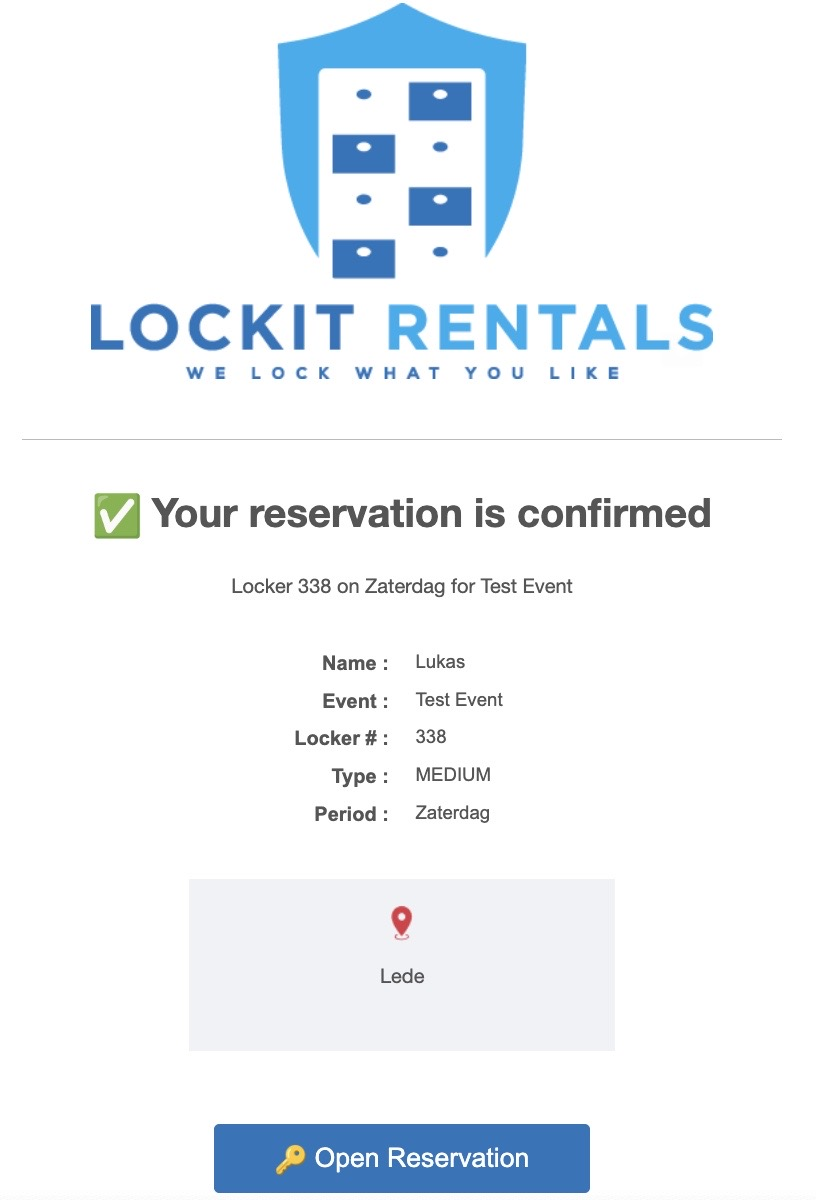
\includegraphics[width=0.5\textwidth]{graphics/F34_mailQR-code.jpg}
    \captionsetup{justification=centering, singlelinecheck=false}
    
    \caption{Een verstuurde mail afkostig van Lockit Rentals met in bijlage de teruggewonnen QR-code.}
    \label{fig:resultatEmailQR-code}
\end{figure}












